%!TEX TS-program = pdflatex
\documentclass[a4paper,12pt,twoside]{article}

\usepackage{mathptmx}
\usepackage{parskip}
\usepackage[top=1.5in,left=1in,right=1in,bottom=1in]{geometry}
%\setlength{\parindent}{0pt}
%\setlength{\parskip}{\the\baselineskip}

% JT: I've commented this out so that we can see page numbers while writin
%\pagestyle{empty} 

\makeatletter
\renewcommand\@makefntext[1]{%
  \parindent 1em\noindent
  \hbox{\@makefnmark}#1}
\renewcommand\large{\@setfontsize\large{14pt}{18}} % For standardizing with the Word template: normally \large is 14.4pt
\makeatother
\usepackage{titlesec}
\titleformat{\subsection}{\normalfont\normalsize}{\thesubsection.}{1ex}{}
\titleformat{\subsubsection}{\normalfont\normalsize}{\thesubsubsection.}{1ex}{}
\titleformat{\section}{\normalfont\normalsize\bfseries}{\thesection.}{1ex}{}
% \titlespacing*{\section}{0pt}{*0}{0pt}
% \titlespacing*{\subsection}{0pt}{\the\baselineskip}{0pt}

\usepackage{natbib} 
%\bibpunct{(}{)}{;}{a}{,}{,}
\bibpunct{(}{)}{,}{a}{,}{,}

\setlength{\bibsep}{0pt} \relax
\setcitestyle{notesep={: },yysep={, }} \relax

\usepackage{linguex,url}
\def\refdash{} % To suppress the dash in (2-a) etc. Defining both as different versions of linguex had different names for this command.
\def\firstrefdash{}


\usepackage{titleps}
\usepackage{lipsum}
\newpagestyle{mystyle}{
\sethead[\thepage][\Author][]{}{\Title}{\thepage}
}
\pagestyle{mystyle}
\author{Hofmann \and de Marneffe  \and Tonhauser}
%\title{Projection variability of clausal complements across different operators}
\title{Projection variability: Is the family of sentences really a family?}
\makeatletter
\newcommand\Author{Hofmann, de Marneffe, and Tonhauser}
\let\Title\@title
\makeatother
%header with author and title

% JT commented out whle editing
%\pagenumbering{gobble} 
%suppresses page numbering in header


%% other packages I added (LH)
% misc formatting
	\usepackage{booktabs}
    \usepackage[export]{adjustbox}
    \usepackage{rotating}

%% bibliography
	\newcommand{\posscite}[1]{\citeauthor{#1}'s (\citeyear{#1})}

 \newcommand{\poscite}[1]{\citeauthor{#1}'s \citeyear{#1}}

% drawing
	\usepackage{graphicx}
	\usepackage{xcolor}


\begin{document}
%%\maketitle
\setlength{\Extopsep}{0pt}
\thispagestyle{empty}

%{\large \textbf{Projection variability of clausal complements across different operators}}
{\large \textbf{Projection variability: Is the family of sentences really a family?}}\footnote{We thank Taylor Mahler for assistance in collecting the data presented here as well as valuable comments. We gratefully acknowledge the National Science foundation grant \#1452674 (to Marie-Catherine de Marneffe, Craige Roberts, and Judith Tonhauser), which provided financial support for this project.}\\
Lisa HOFMANN --- \textit{University of Stuttgart}\\
Marie-Catherine DE MARNEFFE --- \textit{UCLouvain}\\
Judith TONHAUSER --- \textit{University of Stuttgart}\\

\textbf{Abstract.} We present experimental evidence that the projection of the content of clausal complements \textbf{(i)} varies across entailment-canceling operators, \textbf{(ii)} that the effect of operator varies between clause-embedding predicates, and \textbf{(iii)} we extend a result of \citealt{degen_are_2022}, that projection ratings in polar questions do not categorically distinguish factive from nonfactive predicates, to cases with negation, the epistemic possibility modal \textit{perhaps}, and conditional antecedents. The observed variability is not captured by existing theoretical accounts of projection (e.g., \citealt{heim_projection_1983,van_der_sandt_presupposition_1992,abrusan_predicting_2011,schlenker_triggering_2021}). Our results suggest that an analysis must consider interactions between predicates and operators and raise important questions for future research on projection.	

\textbf{Keywords:} Projection variability, entailment-canceling operators, (non)factive predicates. 

\section{Introduction} \label{sec:intro}

    Textbooks typically present the family-of-sentences diagnostic for projection without addressing by-operator variation (e.g., \citealt{chierchia_meaning_1990}). For instance, the clausal complement of \emph{discover} is diagnosed as as projective content, if its content (here: that Julian dances salsa) follows not just from \ref{ex:simple}, but also from its variants in \ref{ex:family}, where \ref{ex:simple} has been embedded under an entailment-canceling operator, such as negation \ref{ex:neg}, polar questions \ref{ex:q}, epistemic possibility modals \ref{ex:mod}, or conditional antecedents \ref{ex:cond}.

    % In formal semantics/pragmatics, the so-called `family of sentences' diagnostic is the standard way of diagnosing whether a content is projective (e.g., \citealt{chierchia_meaning_1990}). For instance, to diagnose the content of the clausal complement of \emph{discover} as projective content, a researcher would typically observe that the content that Julian dances salsa follows not just from \ref{ex:simple}, but also from the family-of-sentences variants of \ref{ex:simple} in \ref{ex:family}, where \ref{ex:simple} has been embedded under an entailment-canceling operator, such as negation \ref{ex:neg}, polar questions \ref{ex:q}, epistemic possibility modals \ref{ex:mod}, or conditional antecedents \ref{ex:cond}.

    % (e.g., \citealt{frege_uber_1892,strawson_referring_1950,kiparsky_fact_1970,karttunen_conventional_1979}).
    
    \ex.\label{ex:simple} Cole discovered that Julian dances salsa.

	\ex. \label{ex:family}
		\a. \label{ex:neg}
			{\bf Negation:} \hfill
			\emph{Cole didn't discover that Julian dances salsa.}
		\b. \label{ex:q}
			{\bf Polar Question:} \hfill
			\emph{Did Cole discover that Julian dances salsa?}
		\c. \label{ex:mod}
			{\bf Modal:} \hfill
			\emph{Perhaps Cole discovered that Julian dances salsa.}
		\d. \label{ex:cond}
			{\bf Conditional:} \hfill
			\emph{If Cole discovered that Julian dances salsa, Logan will be joyful.}
		\z.
	\z.

    However, prior research is suggestive of variation in the effect of different entailment-cancelling operators on projection. For instance, \citet{karttunen_observations_1971} proposed a distinction between English factive predicates (e.g., \textit{regret}) and semi-factives (e.g., \textit{discover}).
    Based on the examples in \Next, he suggested that the CC of true factives projects across all four operators, but that of semi-factives does not always project from under polar questions, modals, or conditionals.\footnote{See \citealt{beaver_have_2010} for naturally occurring examples in which the CCs of factive predicates do not project from under the four operators, thereby calling into question the distinction between factive and semi-factive predicates. For experimental research on the distinction see \citealt{djaerv-etal2016} and \citealt{djarv_cognitive_2018}. We return to this literature in section \ref{s:analysis}.}

    \ex. \citealt{karttunen_observations_1971}: (22, 24--26)
        \a. John didn't \{regret/discover\} that he had not told the truth.
        \b. Did you \{regret/discover\} that you had not told the truth?
        \b. If I \{regret/discover\} later that I have not told the truth, I will confess it to everyone.
        \b. It is possible that I \{regret/discover\} later that I have not told the truth.
        \z.
    \z.

    There have been two experimental investigations of by-operator projection variation. First, the experiment reported in \citet{smith_relationship_2014} investigated projection from under negation and antecents of conditionals for various types of English projective contents. They found that the expressive content of epithets (e.g., \textit{idiot}) and the CC of \textit{know} was more projective under negation than conditionals. In contrast, the content of appositive relative clauses and the preparatory content of \textit{win} showed the opposite pattern, and the existential presupposition of clefts showed no difference. %However, their task involved asking participants how surprised they would be to learn the content under investigation after observing the utterance. Since other factors besides speaker commitment modulate discourse (un)expectedness (see e.g., \citealt{zimmermann_grammatical_2011,tonnis_german_2021}), it is unclear that they (only) measured projection. 
    
    Second, \citet{sieker_projective_2022}  compared the projection of German factives (\textit{wissen} `know', \textit{bereuen} `regret', \textit{ent\-hüllen} `reveal') and semi-factives (\textit{bemerken} `notice', \textit{entdecken} `discover', \textit{herausfinden} `find out') between the four operators in \ref{ex:family}. The results showed that the CCs of the predicates investigated projected more from under negation than the other three operators. contrary to what \citealt{karttunen_observations_1971} suggested, a comparison of factive and semifactive predicates did not reveal that the CCs of factive predicates project more from under polar questions, modals, or antecedents of conditionals than the CCs of nonfactive predicates.

    %They replicated \poscite{smith_relationship_2014} result that the CC of \textit{know} projects more from under negation than conditionals for German \textit{wissen} (`know'). However, this finding was part of an overall pattern of higher projection ratings with negation than other operators.
    %
    %Grouping ratings for the four factive and semi-factive predicates, respectively, they found no interaction of operator with predicate type, and thus no evidence for the factive/semi-factive distinction (iii), or an operator/predicate interaction (ii). However, their analysis did not explore the impact of operators on each predicate individually.

    This paper reports on the results of a set of experiments that were designed to compare projection from under the four entailment-canceling operators in \ref{ex:family}. Our experiments extend the empirical scope of prior research by investigating projection for a broader set of contents, namely the contents of the complements of the 20 English clause-embedding predicates in \ref{ex:predicates}:
    
    \ex. \label{ex:predicates}
    		\a. (Semi)factive predicates: {\em be annoyed, know, reveal, discover, see}
      \b. Nonfactive predicates: {\em acknowledge, admit, announce, confess, confirm, establish, hear, inform, prove, be right, demonstrate, pretend, say, suggest, think}
    
    As shown, the  20 predicates include both (semi)factive and nonfactive predicates. The inclusion of the latter set of predicates is motivated by the results of the empirical investigations in \citealt{degen_are_2022}, which suggested that the contents of complements of nonfactive predicates is also projective and that projection does not categorically distinguish factive and nonfactive predicates. As \poscite{degen_are_2022} result was established based on sentences where the predicates were embedded under polar questions, our experiments, which feature all four entailment-canceling operators, serve to replicate and extend this result of \citealt{degen_are_2022}.

    %    The factive/semi-factive distinction (iii) is further called into question by \citealt{beaver_have_2010}, who reports many naturally occurring examples of cognitive factive predicates, showing that their CC does not necessarily project (e.g., English \emph{be/become aware, know, discover, notice, find out, realize, accept the fact}; French \emph{trouver} \lq discover\rq).

    %Experimental findings from \citet{djarv_cognitive_2018}, \citet{tonhauser_how_2018}, and \citet{degen_are_2022} can be evaluated with respect to whether they support Karttunen's distinction (iii), with mixed results. These studies observed by-predicate variation in polar questions, where more projection is expected for factives than semi-factives.
	%
	%\citet{djarv_cognitive_2018}, assessing acceptability of affirming the main clause while denying the CC, did find higher ratings for English \emph{be happy} and \emph{appreciate} (assumed to be factive) and \emph{be aware} than \emph{realize} (assumed to be semi-factive). This could be interpreted as limited support for (iii). But here, it is also not obvious how exactly this task relates to projection.\footnote{Say why}
	
	%\citet{tonhauser_how_2018} and \citet{degen_are_2022} measured speaker commitments toward the CC of a broad range of English clause-embedding predicates more directly, by collecting judgments of how certain participants take a speaker to be of the contents under investigation.
	%
	%The observed differences between the various predicates do not align with theoretically assumed lexical classes. While \citet{degen_are_2022} demonstrate this for the distinction between purported factive and non-factive predicates, the results did not match the expectations from Karttunen's factive vs. semi-factive classification either.
	%
	%\citet{tonhauser_how_2018} found, e.g., that the CC of semi-factive \emph{realize} was as projective as that of factive \emph{be annoyed} and more than that of semi-factive \emph{discover}. \citet{degen_are_2022} observed that the CC of factive \textit{reveal} was less projective than that of semi-factive \textit{discover}, which, in turn, was less projective than that of factive \textit{know}. These findings also suggest that examining projection ratings for various predicates individually, rather than pre-grouping them based on theoretical assumptions, can provide more nuanced insights into by-predicate projection variation.
    

	%Both \citet{smith_relationship_2014} \citet{sieker_projective_2022} found that projection is affected differently by entailment-cancelling operators. However, while Smith \& Hall found variation in the effect of the operator on projection between various projective contents, Sieker \& Solstad did not.
	%
	%These divergent results raise the question if they are due to cross-linguistic variation, task differences, or artifacts of the analysis. Finally, much previous research calls into question the hypothesis that by-predicate differences in the effect of operator on projection pattern according to Kattunen's factive/semi-factive distinction (\citealt{beaver_have_2010,tonhauser_how_2018,sieker_projective_2022,degen_are_2022}).

  
  %Karttunen's distinction gives rise to three hypotheses about the projection associated with clause-embedding predicates, which we explore in this paper: \textbf{(i) by-operator variation:} entailment-cancelling operators differentially affect projection; \textbf{(ii) operator/predicate interaction:} the effect of operator differs between predicates; \textbf{(iii) factive/semi-factive distinction:} this difference can be addressed by characterizing lexical classes of (semi-)factive predicates.

  
    %To address the three hypotheses, we conducted a set of experiments designed to assess projection across the four entailment-canceling operators in \ref{ex:family} for various clause-embedding predicates. We used the same projection measure as \citet{sieker_projective_2022} (the `certain that' task; see e.g., \citealp{tonhauser_how_2018,djarv_prosodic_2017,mahler_social_2020}) and applied it to the CC of 20 English predicates, including factives and semi-factives, and 15 non-factive predicates, given recent findings that their complements may also project, albeit to varying degrees (\citealt{degen_are_2022}). Our findings support (i) by-operator variation, and an operator/predicate interaction (ii), but not Karttunen's factive/semi-factive distinction (iii).


\section{Experiments}

	To assess the effect of entailment-cancelling operator and clause-embedding predicate on projection, we collected projection judgments for the CCs of the 20 clause-embedding predicates in four sets of experiments.\footnote{The data and analysis scripts can be found in the following GitHub repository: \url{https://github.com/judith-tonhauser/CommitmentBankPlus}. {\bf LETS BE MORE SPECIFIC HERE ABOUT WHERE THINGS RELATED TO THIS PAPER ARE}} The predicates were embedded under negation in Exps.~1, under polar questions in Exps.~2, under the epistemic possibility modal {\em perhaps} in Exps.~3, and in conditional antecedents in Exps.~4. Each set of experiments consisted of three experiments that differed in the at-issueness measure used in a separate block. In this paper, we limit our attention to the projection ratings collected in the 12 experiments.

	Projection was measured in each experiment with the `certain that' diagnostic, which has been used to measure projection with both polar interrogative and declarative sentences (see, e.g., \citealt{tonhauser_prosodic_2016,djarv_prosodic_2017,stevens_rational_2017,lorson_influence_2018,tonhauser_how_2018,mahler_does_2019,mahler_social_2020,de_marneffe_commitmentbank_2019}).\footnote{For other diagnostics of projection see, e.g.\ \citealt{smith_projection_2011,xue_correlation_2011}, and \citealt{tonhauser_toward_2013}; and discussion in \citealt{tonhauser_how_2018}.} This diagnostic was also used in \citealt{sieker_projective_2022}. Under this diagnostic, participants are presented with utterances like those in \Next. They are asked to rate whether the (named) speaker is certain of the CC. 

	\ex. \label{ex:certain-that}
		\a. Christopher: \emph{\lq Cole didn't discover that Julian dances salsa.\rq}
		\b. Christopher: \emph{\lq Did Cole discover that Julian dances salsa?\rq}
		\c. Christopher: \emph{\lq Perhaps Cole discovered that Julian dances salsa.\rq}
		\d. Christopher: \emph{\lq If Cole discovered that Julian dances salsa, Logan will be joyful.\rq}
		\z.
		Projection question: Is Christopher certain that Julian dances salsa?
	\z.

    We assume, following \citealt{tonhauser_how_2018} and \citealt{degen_are_2022}, that judgments of speaker certainty about some propositional content reflect speaker commitment to that content, that is, projection. If a participant interprets an utterance like \Last[a--d] in a way that the speaker (e.g., Christopher) is certain of the CC, it is assumed to project out of the entailment-canceling environment. If a participant does not take the speaker to be certain of the CC, this is taken to indicate that it does not project.

    %This setup allows us to test the three hypotheses outlined in Section \ref{sec:intro}. First, a main effect of operator on speaker certainty judgments for embedded contents would provide evidence for by-operator variation (i). Second, if there is a operator/predicate interaction (ii), we would expect the effect of operator to be different (in magnitude or direction) for different predicates. Finally, based on the factive/semi-factive distinction (iii), we would expect the CC of semi-factive predicates to receive high projection ratings under negation and lower ratings under the other operators, while the CC of factive predicates would consistently receive relatively high projection ratings throughout.


	\subsection{Methods}

		\subsubsection{Participants}
			We recruited 250-300 participants for each of the 12 experiments. Participants for Exp.~1q were recruited on Amazon's Mechanical Turk platform; the participants were required to have U.S.\ IP addresses and at least 99\% of previously approved HITs. Participants for the remaining experiments were recruited on Prolific; these participants were required to reside in the US, to be born in the US, to have English as their first language, and to have an approval rating of at least 99\%. See Supplement \ref{app:d-participants} for further information about the participants. 
			

		\subsubsection{Materials}

            The target sentences consisted of 400 combinations of the 20 clause-embedding predicates in \ref{ex:predicates} with 20 embedded clauses (provided in Supplement \ref{app:a-clauses}). As mentioned above, the predicates were embedded under negation in Exps.~1, under polar questions in Exps.~2, under the epistemic possibility modal \emph{perhaps} in Exps.~3, and in conditional antecedents in Exps.~4, for a total of 400 target stimuli in each of the four sets of experiments. 
  
			%We tested the 20 clause-embedding predicates in \Next, which have shown projection variability in polar questions (\citealt{degen_are_2022}). They comprise three factive predicates \Next[a], two semi-factives \Next[b], nine that have been characterized as optionally factive in \citealt{kiparsky_fact_1970} \Next[c], and six non-factives which include two veridical predicates \Next[d], and four non-veridical ones \Next[e].

	%		\ex. 20 clause-embedding predicates \hfill \citealt{degen_are_2022}
			%	\a. canonically factive:					\emph{be annoyed, know, reveal}
				%\b. semi-factive: 		\emph{discover, see}
%				\b. optionally factive: \newline \emph{acknowledge admit, announce, confess, confirm, establish, hear, inform, prove}
%				\b. Non-factive veridical:
%					\emph{be right, demonstrate}
%				\b. Non-factive non-veridical:
%				\emph{pretend, say, suggest, think}
%				\z.
%			\z.

To assess whether participants were attending to the task, each experiment included six control stimuli. For details on the six control stimuli see Supplement \ref{app:c-control}.

Each participant saw a random set of twenty-six stimuli: Each set contained one target stimulus for each of the 20 clause-embedding predicates (each with a unique complement clause) and the same six control stimuli.\footnote{Each participant saw their set of 26 stimuli twice, once in the projection block and once in the at-issueness block. Block order was randomized. As mentioned above, we focus on the projection ratings here.} Trial order was randomized.
  
  
  %which were main clauses with appositive relative clauses, which were also presented as utterances made by a named speaker. Here, the main clause content was targeted by the projection question. In the experiments with polar questions, the controls were expected to receive low certainty ratings, whereas in the experiments with declaratives, they were expected to receive high ratings.

  %Each participant saw all 20 predicates, randomly paired with a unique embedded clause from a set of 20 contents, and a subject from a set of 20 proper names. %The predicates associated with projective content were embedded under (i) negation, (ii) polar questions, (iii) the epistemic possibility modal \textit{perhaps}, and (iv) in conditional antecedents in the four different sets of experiments.

		
        \subsubsection{Procedure}

			Participants were told to imagine that they are at a party and that, on walking into the kitchen, they overhear somebody say something to somebody else.
            %
            On each trial, participants read an utterance and responded to the `certain that'   question. They gave their response on a slider marked `no' (coded as 0) at one end and and `yes' (coded as 1) on the other. A sample trial from Exps.~1 is illustrated in Figure~\ref{fig:trial}. Following, e.g., \citet{tonhauser_how_2018}, higher ratings of speaker certainty could reflect one of two things:
            %
            On the one hand, higher ratings could reflect greater speaker commitment towards the CC, and therefore greater projection. This assumes that projection (and the relevant notion of speaker commitment) can itself be gradient.
            %
            Conversely, higher ratings could also reflect the probability that a participant associates with a projective interpretation for the utterance. Under this interpretation, commitment may be interpreted categorically, and the gradience is a result of the uncertainty about possible interpretations (see also discussion in \citealt{grove_factivity_2023}, which suggests the latter kind of interpretation).

            %  we take high ratings of speaker certainty to reflect speaker greater speaker commitment towards the CC, that is, greater projection.

			\begin{figure}[ht]
				\centering
				\fbox{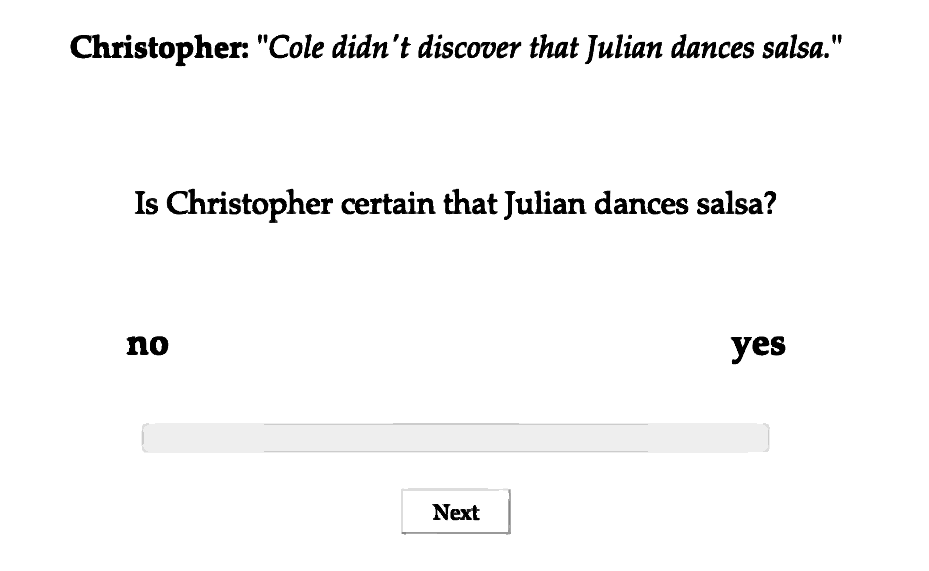
\includegraphics[width = .7\linewidth]{task-1n-proj.eps}}
				\caption{A sample trial in Exps.~1. In the corresponding trials in Exps.~2-4, participants were presented with an utterance with a different entailment-cancelling operator.}
				\label{fig:trial}
			\end{figure}
   
             After completing the experiment, participants filled out a short optional demographic survey. To encourage truthful responses, participants were told that they would be paid no matter what answers they gave in the survey.

        \subsubsection{Data exclusion}

        Data were excluded based on self-declared non-native speaker status and other criteria given in the Supplements \ref{app:d-participants}. The data from 2,682 participants entered into the analysis.  

            %We analyze the data from $2,682$ self-reported native speakers of American English, after excluding participants who failed one of the following two attention-checks: their mean rating on six control items is more than 2 sd different from the group mean, or they always roughly selected the same point on the scale for target stimuli (identified by low variance, and then manually inspecting their response patterns).

    \subsection{Results and discussion}

    We first address the question of whether there is by-operator variation (section \ref{s:by-op}) and then the question of whether there is by-predicate variation in the observed by-operator variation (section \ref{s:by-pred}).
    
		%Our data reveals three key results: \textbf{(i)} There is projection variability by operator; \textbf{(ii)} There is by-predicate variation in the effect of operator on projection; and \textbf{(iii)} We find further support (from entailment-cancelling operators beyond polar questions) for \posscite{degen_are_2022} result that by-predicate projection variation is gradient in a way that cannot be predicted by categorical lexical classes.
		
	\subsubsection{By-operator variation}\label{s:by-op}

        Fig.~\ref{fig:op-ratings} shows the mean certainty ratings by entailment-canceling operator, aggregating over the clause-embedding predicates. As shown, there is projection variability by operator: The CCs of the clause-embedding predicates were relatively more projective when embedded in the antecedent of a conditional than in a polar interrogative, where they were relative more projective than when they were embedded under negation or the epistemic modal {\em perhaps}.
  
			%When aggregating across predicates, we found an effect of \texttt{operator}. The distribution of projection ratings, as well as means and $95\%$ bootstrapped confidence intervals by operator are shown in Figure~\ref{fig:op-ratings}.

			\begin{figure}[ht]
				\centering
				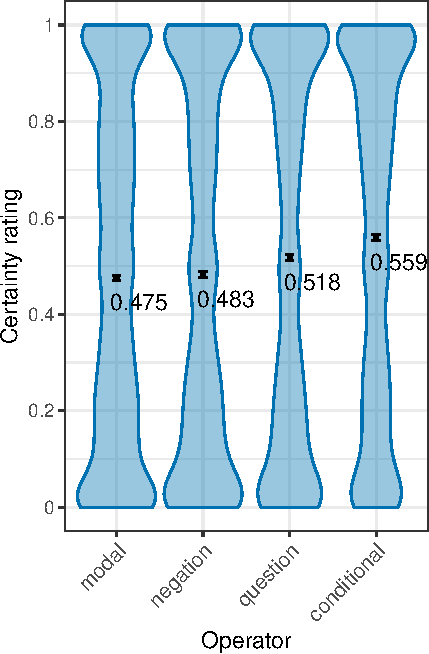
\includegraphics[scale = .8]{operator-graph-1}
				\caption{Mean certainty ratings by operator. Error bars indicate $95\%$ bootstrapped confidence intervals. Violin plots indicate the kernel probability density of the individual participants’ ratings.}
				\label{fig:op-ratings}
			\end{figure}

			%Mean projection ratings were higher for CCs in question-embeddings than under negation and modals, but lower than in conditional antecedents. 
   
   These generalizations are supported by Model \#1 reported in Table~\ref{t:op-model}.

			\begin{table}[ht]
					\centering
					\hspace{-1.3em}
					\begin{tabular}{llrrrr}
						Model & & Estimate & Std. Error & t-value\\
						\midrule
						\#1 & Intercept: \emph{question} & 0.51 & 0.01 & 44.78 & ***\\
						& operator: conditional & 0.05 & 0.01 & 5.30 & ***\\
						& operator: modal & -0.04 & 0.01 & -4.45 & ***\\
						& operator: negation & -0.03 & 0.01 & -4.67 & ***\\
						\bottomrule
					\end{tabular}
				
					\caption{Excerpt from the model output of a linear mixed effects model with fixed effects of operator; random effects: participant and item intercepts, fitted with \texttt{lme4, lmertest} in \texttt{R}.\label{t:op-model}}
				\end{table}

			Like \citet{sieker_projective_2022}, we observe a small main effect of entailment-cancelling operator on projection. However, in contrast to their result that projection is strongest from under negation, our results suggest that projection is strongest from antecedents of conditionals.
            We note, however, that the differences in mean certainty ratings between the four entailment-canceling operators are very small. This suggests that, when abstracting away from individual projective contents, projection from under the four entailment-canceling operators is very similar. In other words, when abstracting away from individual projective contents, the family of sentences really are a family.


		\subsubsection{By-predicate variation in the effect of entailment-canceling operator}\label{s:by-pred}

  Fig.~\ref{fig:op-pred-ratings} shows mean certainty ratings by predicate and entailment-canceling operator (aggregating over the 20 CCs that each predicate was paired with). As shown, there is by-operator variation for the CCs of all 20 clause-embedding predicate, that is, there is not a single predicate for which there is no by-operator variation. The observed variation does not align with widely assumed predicate classes. For instance, the five (semi)factive predicates exhibit five different patterns: 
i) the CC of \emph{be annoyed} projects more from under negation and questions than conditionals and modal {\em perhaps}; ii) the CC of \emph{know} projects most from under questions, less from questions and negation, and least from under the modal {\em perhaps}; iii) the CC of \emph{see} projects most from under questions and conditionals, less from under negation, and least from under the modal \emph{perhaps}; iv) the CC of  \emph{discover} projects more from under conditionals and questions than negation and modal {\em perhaps}; and v) the CC of \emph{reveal} projects most from conditionals, less from questions, and least from negation and modal \emph{perhaps}. Thus, contrary to what \citealt{karttunen_observations_1971} proposed, there is no predicate whose CC projects uniformly from under all four entailment-canceling operators (as he suggested for factive predicates) and the purported semi-factive predicates  \emph{discover} and \emph{reveal} do not project more from under negation than the other three entailment-canceling operators. We also observe by-operator projection variation for nonfactive predicates. Some of this variation aligns with that observed for factive predicates: For instance, the CC of \emph{inform} exhibits the same pattern as the CC of \emph{know}, and the CC of \emph{acknowledge} exhibit the same pattern as that of the CC of \emph{discover}. Other nonfactive predicates exhibit other patterns: For instance, the CCs of \emph{admit}, \emph{confess} and \emph{announce} project most from the antecedents of conditionals than the other three operators. 

\begin{figure}[ht]
				\centering
				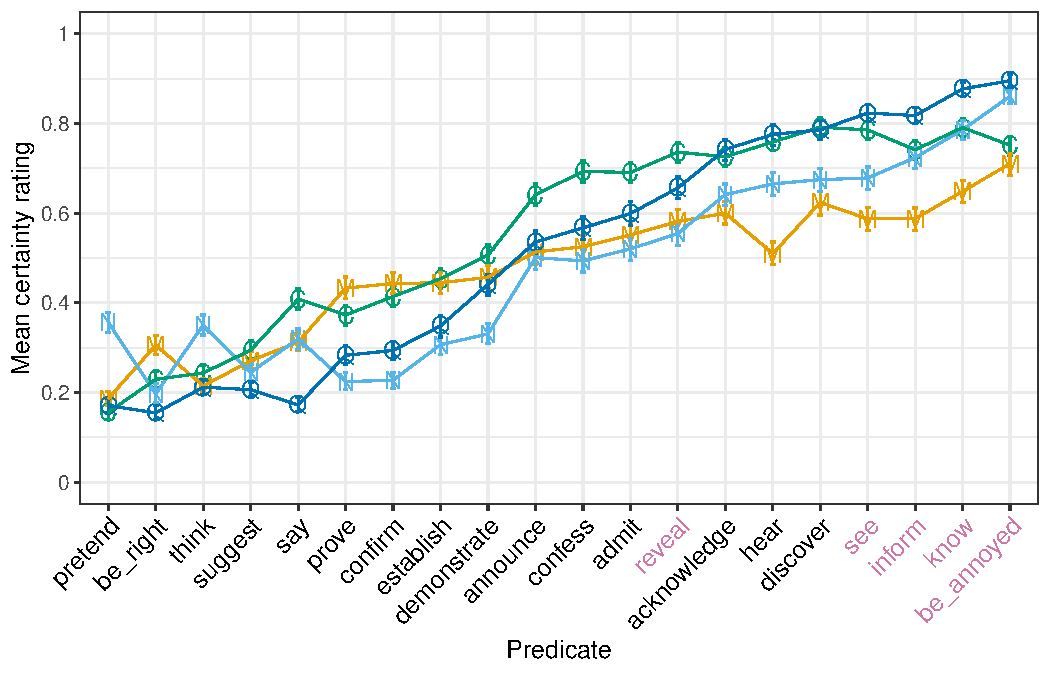
\includegraphics[width = \linewidth]{predicate-operator-graph-1}
				\caption{Mean certainty ratings by predicate and operator with 95\% bootstrapped confidence intervals. Predicates are ordered by mean certainty rating pooled over the four operators.
Embedding operator coded by letter and color:  \texttt{N} (light blue): negation, \texttt{M} (orange): modals, \texttt{C} (green): conditional antecedents, \texttt{Q} (dark blue): polar questions.}
				\label{fig:op-pred-ratings}
			\end{figure}

The observation that there is by-operator variation for the CC of each of the 20 clause-embedding predicates is confirmed by the statistical analysis. We fitted...
    
  The CC of \emph{know} projects less from under negation than questions, but more from under negation than modals, while the difference between negation and conditionals is not significant.
			%
			These generalizations are supported by models\ \# 2--4 in Table\ \ref{t:models}, which also each have at least $34$ highly significant interaction terms (out of $57$ possible interactions of operator and predicate).

			\begin{table}[ht]
				\centering
				\begin{tabular}{llrrrr}
					Model & & Estimate & Std. Error & t-value\\
					\midrule
					\#2 & Intercept: \emph{\bf be annoyed}/negation & 0.87 & 0.01 & 79.86 & ***\\
					& operator: conditional & -0.12 & 0.02  & -7.36 & ***\\
					& operator: modal & -0.16 & 0.02  & -10.01 & ***\\
					& operator: question & 0.02 & 0.01 & 1.72 & n.s.\\
					\midrule
					\#3 & Intercept: \emph{\bf discover}/negation & 0.68 & 0.01 & 62.70 & ***\\
					& operator: conditional & 0.11 & 0.02 & 7.11 & ***\\
					& operator: modal & -0.06 & 0.02 & -3.63 & ***\\
					& operator: question & 0.10 & 0.01 & 7.08 & ***\\
					\midrule
					\#4 & Intercept: \emph{\bf know}/negation & 0.79 & 0.01 & 72.97 & ***\\
					& operator: conditional & 0.00 & 0.02 & -0.06 & n.s.\\
					& operator: modal & -0.14 & 0.02 & -9.18 & ***\\
					& operator: question & 0.08 & 0.01 & 5.67 & ***\\
					\bottomrule
				\end{tabular}
				\caption{\small Excerpt of the output from three linear mixed effects models, with fixed effects: operator, predicate, and their interaction; random effect: participant intercepts.
				Models were fit with \texttt{lme4, lmertest} in \texttt{R}. Models \textbf{\#2--4} also had at least $34$ highly significant interaction terms of \texttt{operator} and \texttt{predicate} with $p < 0.001$ (not shown here).\label{t:models}}
			\end{table}

Our results align with those of \citealt{smith_relationship_2014}, who also observed by-expression by-operator variation. However, while they found that the CC of \emph{know} projects more from under negation than the antecedent of a conditional, we did not find an effect here. We hypothesize that this difference is due to the difference in projection diagnostic used. 

			%Our result that by-operator projection variability interacts with predicate concurs with \citet{smith_relationship_2014}, while we did not reproduce their result that the CC of \emph{know} projects more from negation than conditionals (we found no difference here). 
   Our results differ from those of \citealt{sieker_projective_2022}: While that work did not find differences in by-operator projection variation between factive and semi-factive predicates, our results suggested five different patterns of by-operator variation for the five (semi)factive predicates. As \citealt{sieker_projective_2022} also used the `certain that' diagnostic for projection, this difference in results is not likely due to the diagnostic. Other factors that varied between our experiments are the language under investigated (German vs.\ English), the clause-embedding predicates investigated, and the CCs that the predicates were paired with. Future research will need to establish which of these factors are implicated in the observed differences.
   
%   , who found no difference between the two groups of predicates they assumed in the effect of operator.
			%
			%However in line with Sieker \& Solstad, our results question \posscite{karttunen_observations_1971} proposed difference between factive and semi-factive predicates (see also \citealt{beaver_have_2010}). Although our data replicate the result from \citet{tonhauser_how_2018} that, in polar questions, the CC of semi-factive \emph{discover} is less projective than that of \emph{know}, the same does not hold in conditionals, contrary to what would be expected based on \posscite{karttunen_observations_1971} distinction between factive and semi-factive predicates.
			%
			%Further, the CC of (factive) \emph{be annoyed} does not project invariably from all four operators, and the CC of \emph{discover,}  which is considered semi-factive, does not project more from under negation than the other three operators. The pattern observed for {\em know} does not fit into either category.

	\subsubsection{Factive vs.\ nonfactive predicates}

Factive predicates are defined as predicates that presuppose the CC, while the CC of nonfactive predicates is not presupposed (e.g., \citealt{kiparsky_fact_1970,karttunen_observations_1971,schlenker_local_2010,abrusan_predicting_2011}).\footnote{Some of these works additionally assume that the CC of factive predicates is entailed.} As presuppositions are assumed to project from under entailment-canceling operators, this definition leads one to expect that factive predicates are distinguished from nonfactive ones by the projection of their CCs: The CCs of factive predicates are expected to be categorically more projective than those of nonfactive ones. This expectation was investigated in \citealt{degen_are_2022} based on the 20 clause-embedding predicates in \ref{ex:predicates}, which were embedded in polar questions. Contrary to expectation,  \citealt{degen_are_2022} found variation among the CCs of the five factive predicates investigated and that the CCs of some nonfactive predicates were as projective, or even more projective, than the CCs of some factive predicates.  In short, projection of the CC from under polar questions did not categorically distinguish factive from nonfactive predicates.

The results of the set of experiments reported on in this paper replicate this result. As shown in Fig.~\ref{fig:op-pred-ratings}, there is variation between the CCs of the five factive predicates in the polar question condition, and projection from under polar questions does not categorically distinguish factive from nonfactive predicates. Furthermore, the results of  this set of experiments suggest that projection from under the three other entailment-canceling operators also does not categorically distinguish factive and nonfactive predicates. This result strengthens the conclusion of \citealt{degen_are_2022} that there is, to date no empirical evidence for a coherent class of factive predicates.

IF THERE IS ROOM I WOULD LIKE TO INCLUDE 4 VERSIONS OF FIG 3 WHERE THE 20 PREDICATES ARE ORDERED BY OPERATOR, TO MAKE THE POINT OF THIS SECTION CLEARER. THAT WOULD ALSO BE GOOD FOR THE METHODOLOGICAL IMPLICATION SECTION BELOW.

		Modal:\newline
		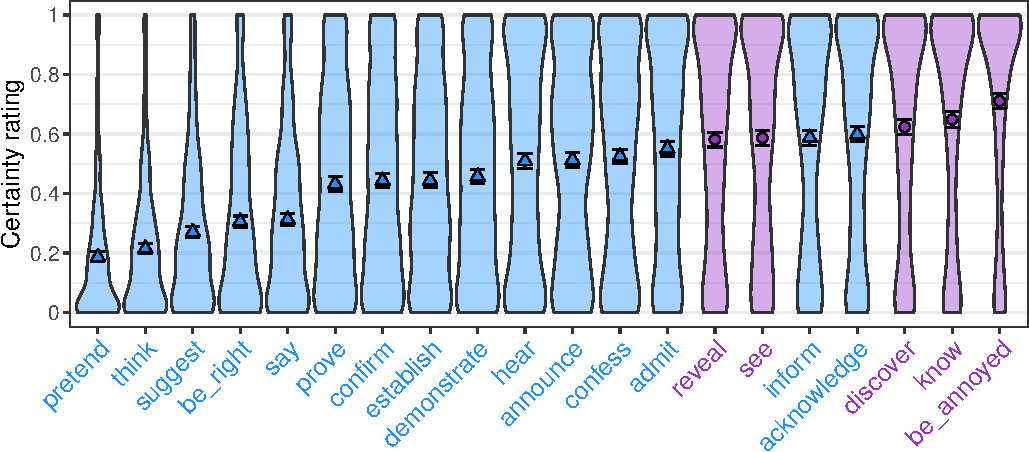
\includegraphics[width = \linewidth]{modal-predicate-graph-1.pdf}
        Negation:\newline
        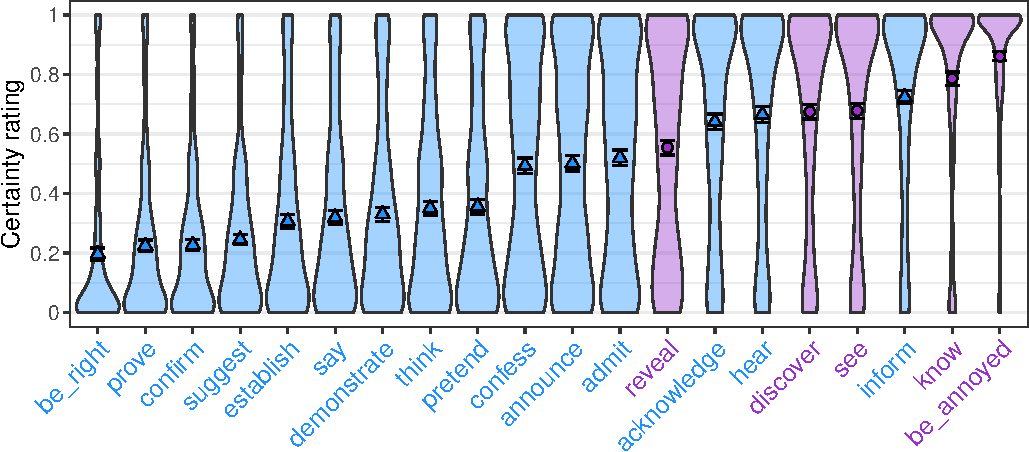
\includegraphics[width = \linewidth]{negation-predicate-graph-1.pdf}
        Polar questions:\newline
        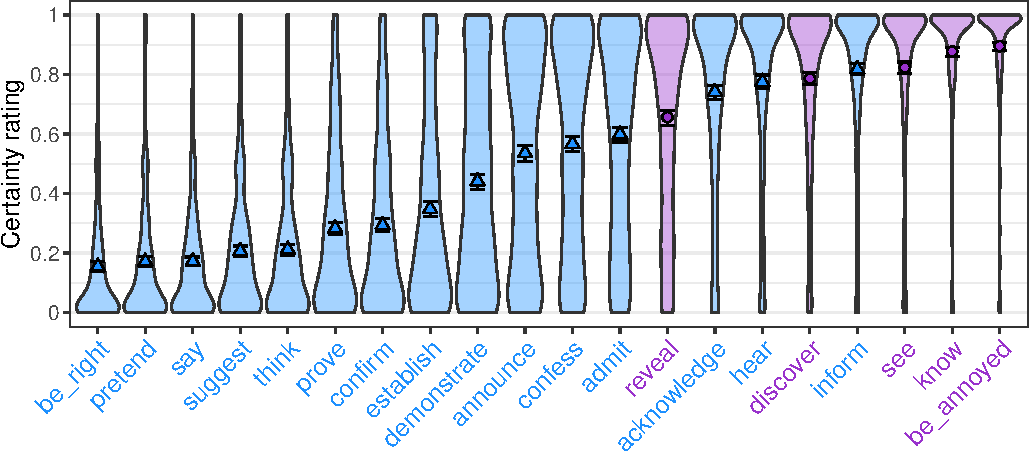
\includegraphics[width = \linewidth]{question-predicate-graph-1.pdf}
        Conditionals:\newline
        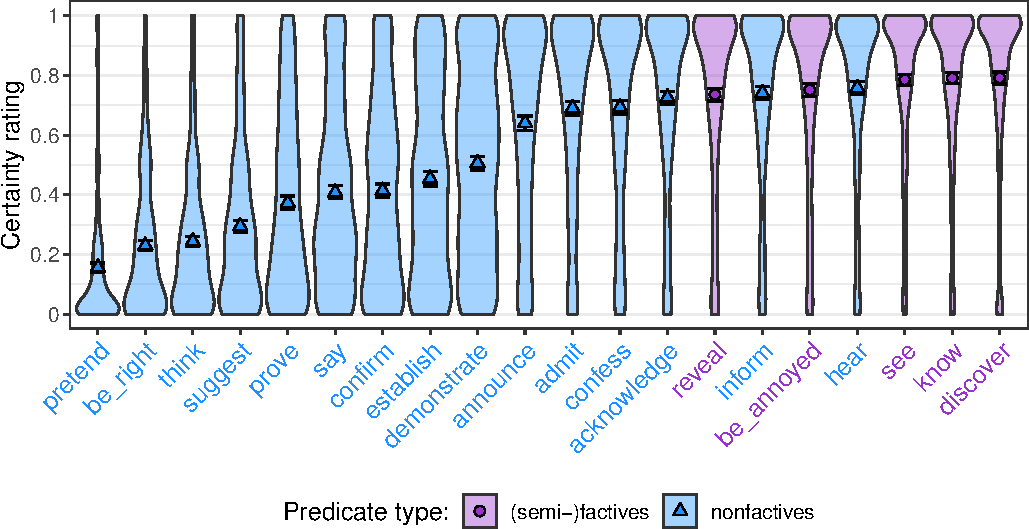
\includegraphics[width = \linewidth]{conditional-predicate-graph-1.pdf}
		%\caption{Mean certainty ratings by predicate, for each operator. Error bars indicate $95\%$ bootstrapped confidence intervals. Violin plots indicate kernel probability densities of individual observations.}

    

%			Taking into account the effect of \texttt{predicate} on projection, we find gradient projection variation, like \citet{tonhauser_how_2018} and \citet{degen_are_2022}.
			%
			%This is illustrated in Figure~\ref{fig:op-pred-ratings}, which shows mean projection ratings for the 20 predicates grouped by embedding operator. Here, predicates on the x-axis are ordered by their mean rating across all operators (\emph{be annoyed} has the highest overall mean).

			

			%Our results therefore provide further support from negation, modals, and conditionals for the result of \citet{degen_are_2022}, that projection does not categorically differentiate between (semi-)factive and non-factive predicates, while also replicating it for polar questions. The CCs of non-factive \emph{inform} and \emph{acknowledge}, for instance, are at least as projective as that of some (semi-)factive predicates.

   
		\subsubsection{Summary}

  The results of our experiments suggest that there is little by-operator variation when aggregating over clause-embedding predicates, but that the CCs of different clause embedding predicates exhibit by-operator projection variation. 
			%Based on our data, we conclude that embedded propositional content projects differently from under different entailment-cancelling operators. 
    Crucially, the observed by-operator variation does not align with prior claims about differences between factive and semi-factive predicates in by-operator variation (e.g., \citealt{karttunen_observations_1971}). Finally, the results of our experiments provide further support for the results of \citealt{degen_are_2022}, who did not find empirical support for a class of factive predicates based on the projection of the CC from under polar questions. Our experiments suggest that projection of the CC from under negation, the antecedent of conditionals and epistemic modals also do not provide empirical support for a natural class of factive predicates.

    Before discussing the methodological and theoretical implications of these results in section \ref{s:general}, we provide converging evidence from a different dataset in section \ref{s:converging}.
   
%   does not categorically distinguish between lexical classes (e.g., factives, semi-factives, veridical predicates), so future research appealing to these categories must clarify their definition.
			%
			%Finally, the effect of operator on projection differs by predicate. The theoretical implications of our findings are discussed in the following section. Importantly, accounts of projective content need to take into account predicate/operator interactions, and the gradient by-predicate variability.
   
		\section{Converging evidence for the by-operator variation}\label{s:converging}

This section provides converging evidence for the by-operator variation based on the MegaVeridicality dataset (\citealt{white_role_2018}). This dataset contains projection ratings for the CCs of 517 English clause-embedding predicates. The stimuli that participants rated consisted of combinations of these predicates with what White and Rawlins (2018) referred to as ‘low content arguments’, as shown in \Next for \emph{know}. The predicates were embedded under negation in stimuli like \Next[a], in the antecedent of a conditional and a polar question in stimuli like \Next[b], and under negation, in the antecedent of a conditional, and in a question in stimuli like \Next[c]. To assess projection, participants were asked to respond to the question \emph{Did that thing happen?} for stimuli like \Next[a] and to respond to the question posed by stimuli like \Next[b] and \Next[c]. The response options were ‘yes’, ‘maybe or maybe not’, and ‘no’.

			%Our experimental result that that the effect of entailment-cancelling operator differs by predicate finds further support in the data from \posscite{white_role_2018} MegaVeridicality dataset.
			%
			%White \& Rawlins assess projection inferences associated with 517 clause-embedding predicates by presenting them in 50 \lq low-content\rq\ syntactic frames, like the ones in \Next, illustrated here with \textit{know}. The frames in \Next present predicates associated with projective contents embedded under negation \Next[a], in conditional antecedents \Next[b], or both \Next[c], in combination with a projection question (\textit{Did that thing happen?}).

			\ex. \a. Somebody didn’t know that a particular thing happened. Did that thing happen?
				\b. If somebody knows that a particular thing happened, did that thing happen?
				\b. If somebody didn’t know that a particular thing happened, did that thing happen?
				\z.
			\z.

To investigate by-operator projection variability, we recoded `yes' responses as 1, `no' responses as -1, and `maybe or maybe not' responses as 0. We then calculated the mean projection rating for 16 predicates under the three types of operator combinations shown in \Last. The 16 predicates include ones also used in our experiment as purported factives (\textit{be annoyed, know, reveal}) and semi-factives (\textit{discover, see}), and eleven further predicates commonly characterized as factive or semi-factive (\textit{amuse, find out, forget, learn, love, notice, realize, recognize, regret, remember, understand}).

			%In a series of experiments, participants presented with stimuli like \Last responded with \lq yes\rq, \lq no\rq, or  \lq maybe\rq (coded as \texttt{1, -1,} or \texttt{0}, respectively). Here, we present data from their data set, for the frames in \Last, and 16 of their predicates. These include ones also used in our experiment as purported factives (\textit{be annoyed, know, reveal}) and semi-factives (\textit{discover, see}), and eleven further predicates commonly characterized as factive or semi-factive (\textit{amuse, find out, forget, learn, love, notice, realize, recognize, regret, remember, understand}).

			The mean projection ratings by embedding context and predicate are presented in Figure~\ref{fig:figure4}, which shows that effect of embedding context on projection differs by predicate.

			For instance,\footnote{Give some examples of differences here, but first double check if lines are labeled correctly. Also angle labels on x-axis.}

			% the predicates \textit{see} and \textit{learn} have the same mean ratings for both negative and conditional contexts. However, the effect of negative conditional contexts does not simply reflect the additive result of both effects, but 

			\begin{figure}[ht]
				\centering
				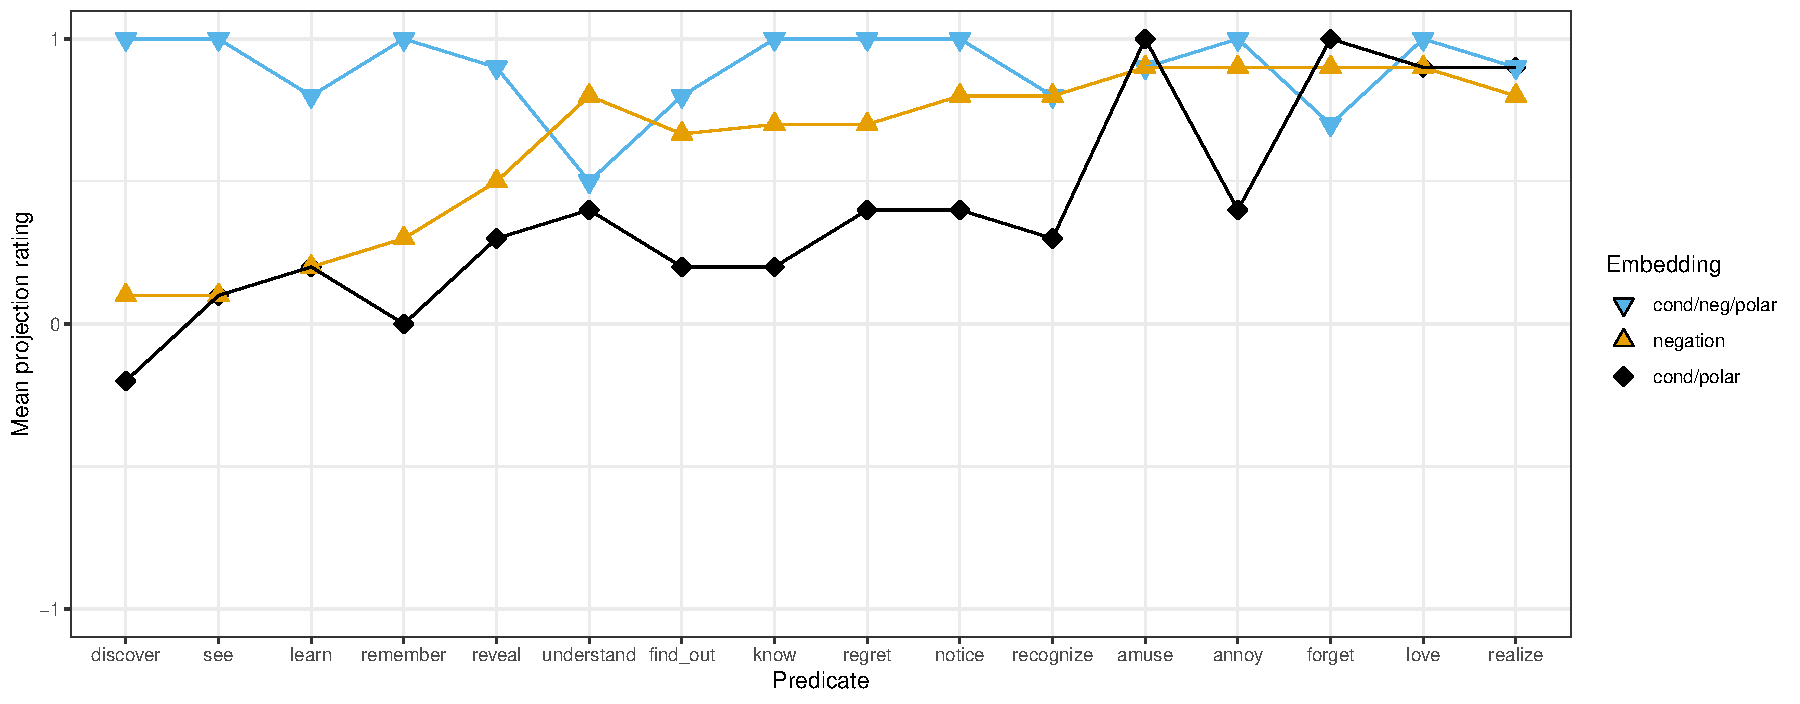
\includegraphics[width = \linewidth]{mega-veridicality}
				\caption{Mean projection ratings by embedding context and predicate.}
				\label{fig:figure4}
			\end{figure}

			It is worth noting that the task assesses global projection only in case of \Last[a], but not \Last[b+c], where the question \textit{did it happen?} is embedded in the conditional consequent. It assesses whether the projective inference holds in the conditional local context. Nevertheless, the data provides supporting evidence for by-predicate variation in the effect of operators on projection. Crucially, the by-predicate variation in the effect of negation in the global context is different from the by-predicate variation in the effect of negation in the conditional context.


\section{General discussion}\label{s:general}

In this section, we point out methodological implications of our results (section \ref{s:method-impl}), discuss whether contemporary projection analyses can capture the observed variation (section \ref{s:analysis}), and speculate about lexical differences between the clause-embedding predicates that might predict the by-operator variation observed (section \ref{s:lex}).

\subsection{Methodological implications}\label{s:method-impl}

A methodological implication of this latter result is that future research must relativize claims about projection variation to the entailment-canceling operator.

\subsection{Theoretical implications}\label{s:analysis}

In this section, we consider whether contemporary analyses can capture the observed by-predicate projection variation and the interactions between predicate and entailment-canceling operator in projection ratings. We consider three types of analyses: (i) analyses that assume that the CCs of factive predicates are lexically specified as presupposed  (\citealt{heim_projection_1983,heim_presupposition_1992,van_der_sandt_presupposition_1992}), (ii) analyses on which backgrounded entailments are projective (\citealt{abrusan_predicting_2011,simons_best_2017}), and (iii) an analysis on which contextual entailments are projective 
%with a triggering algorithm based on world-knowledge that operates over contextual entailments of an utterance 
(\citealt{schlenker_triggering_2021}). 

%While all of these approaches meet limitations in accounting for our data, we argue that the observed gradient effects of predicate/operator interactions favor integrating insights from competing accounts, namely a contextual triggering algorithm (as in \citealt{abrusan_predicting_2011,simons_best_2017}) operating over contextual set of inferences (as in \citealt{schlenker_triggering_2021}).
	

	%Our results---that projection is modulated by entailment-canceling operators and that there is by-predicate variation in the effect of operator on projection---are not captured by contemporary projection analyses.

\subsubsection{Analyses on which presuppositions are lexically specified}

On the analyses in \citealt{heim_projection_1983,heim_presupposition_1992} and \citealt{van_der_sandt_presupposition_1992}, the CCs of factive predicates are lexically specified as presupposed, in contrast to the CCs of nonfactive predicates. Presupposed CCs project to the global context, except when that would produce an inconsistency, in which case they are accommodated to the local context of the operator.

\paragraph{By-predicate variation.} Analyses on which some clause-embedding predicates are factive and others are nonfactive do not predict the observed by-predicate variation, for several reasons. One reason is that there is variation between the factive predicates: For instance, the CC of \emph{be annoyed} is more projective than that of \emph{discover}, which in turn is more projective than that of \emph{reveal}. This variation is not predicted because the CCs of factive predicates are invariably specified as presupposed. The variation is also not predicted because, in our experiment, the stimuli were presented in minimal contexts that were not inconsistent with the CCs, thereby rendering local accommodation unlikely. A second reason is that the CCs of some nonfactive predicates (e.g., \emph{inform, acknowledge})  are just as projective as those of some factive predicates, or even more projective. Analyses like those in \citealt{heim_projection_1983,heim_presupposition_1992} and \citealt{van_der_sandt_presupposition_1992} fail to make predictions about the projection of the CCs of nonfactive predicates. Thus, as discussed in detail in \citealt{degen_are_2022}, the factive/nonfactive distinction is not sufficiently fine-grained to adequately predict the observed by-predicate projection variation.

%The assumption of categorical lexical triggering does not address the projection variation among purported factive predicates (see also discussion in \citealt{degen_are_2022}). It also cannot address the fact that the CCs of some non-factive predicates (e.g., \emph{inform, acknowledge}) project just as much, or more, than some (semi-)factive predicates (e.g., \emph{reveal, discover, see}). That is because, it only makes predictions for the projection of the CC of (semi-)factive predicates, whose CCs are analyzed as presuppositions. It therefore does not address the data for the non-veridical predicates in our study.
		%
%		Further, the categorical lexical distinctions are not sufficiently fine-grained to make predictions about the gradient by-predicate variation in the effect of operator on projection.
		%
%		This interaction effect can only be addressed by taking into account more fine-grained lexical distinctions than assuming that some predicates are presuppositional, while others are not.


	\paragraph{By-operator variation.} 
        %In our experiment, the stimulus utterances were presented out of the blue, leaving it to the participants to imagine a suitable discourse context. Therefore, none of the CCs should be interpreted as necessarily inconsistent with contextual information.
		%
		The analyses in \citealt{heim_projection_1983,heim_presupposition_1992} and \citealt{van_der_sandt_presupposition_1992} do not lead us to expect differential effects of entailment-cancelling operators on projection. This is because negation and conditional antecedents are given a semantics that derives their behavior as presuppositional \lq holes\rq\ (in the sense of \citealt{karttunen_observations_1971}). For instance in \citealt{heim_projection_1983}, presupposition triggers under negation or in conditional antecedents are evaluated relative to the global context set. Therefore, presupposition triggers under these operators are predicted to behave like unembedded ones, with no expected differences. While the analyses does not explicitly address epistemic possibility modals or polar questions, we might expect that they would be treated as presuppositional holes along the same lines, therefore also not predicting the observed projection variation.
		%
		%Differential effects of operators on projection could conceivably be addressed in such a system by assuming that the meaning of entailment-cancelling operators systematically affects the possibility of local accommodation (e.g., by assuming that accommodation is more likely under modals than conditional antecedents). However, no such effects have been spelled out.
		
	

	\subsubsection{Analyses on which backgrounded entailments are projective} 
 
		\citealt{abrusan_predicting_2011,abrusan_presupposition_2016} and \citealt{simons_best_2017} do not assume that presuppositions are lexically specified but rather that those entailments that are backgrounded with respect to the discourse context in which the utterance is made may project. %assume that projection is not determined lexically, but by a triggering mechanism, which operates over the entailments of an expression, and determines which of them projects. They assume entailments project that do not contribute to the main point invoked by the utterance.
		% Instead of assuming that the possibility of projection is determined lexically, the accounts in \cite{abrusan_predicting_2011,simons_best_2017} and \citet{schlenker_triggering_2021} assume a triggering mechanism, which operates over a set of inferences associated with an utterance, and determines which of them projects. The assumed triggering mechanisms differ on two dimensions: (i) how the set of inferences is determined that constitutes the input to the triggering mechanism, and (ii) the algorithm by which these inferences are derived as projective or not.
		In \citealt{abrusan_predicting_2011} and \citealt{abrusan_presupposition_2016}, an entailment is backgrounded if it is about a time that is not the event time of the matrix predication and it is not at-issue with respect to the Question Under Discussion (QUD, see \citealt{roberts_information_1996,roberts_information_2012}). In \citealt{simons_best_2017}, an entailment is backgrounded if it is not at-issueness relative to the QUD and not conventionally marked as at-issue.
		%
		%In such analyses, every utterance addresses a question, which is determined by its alternative-structure, which, can be indicated by focus-marking. For example, in a modalized utterance with \emph{be annoyed}, the CC can be focused \Next[b], which leads to the alternative structure in \Next[c], allowing the utterance to address a question like \Next[a].

		%\ex. \a. What was Cole annoyed about today?
		%	\b. Perhaps Cole was annoyed [$_F$ that Julian dances salsa].
		%	\b. $\{p \mid \exists q(p = \lambda w.$\emph{Cole was annoyed that} $q$ \emph{in} $w)\}$
		%	\z.
		%\z.

		%In contrast, focus on the subject \Next[b] leads to the alternative structure in \Next[c], allowing the utterance to address a question like \Next[a].

		%\ex. \a. Who was annoyed today?
		%	\b. Perhaps [$_F$ Cole] was annoyed that Julian dances salsa.
		%	\b. $\{p \mid \exists x(p = \lambda w.x$ \emph{was annoyed in} $w$ \emph{that Julian dances salsa}$)\}$
		%	\z.
		%\z.

		%The account assumes that an inference projects if it is entailed by the union of the alternatives (see also \citealt{abusch_presupposition_2010}). therefore predicting projection of the CC in \Last, but not \LLast. That is, under the assumption that $x$ \emph{was annoyed that} $p$ entails $p$.

		\paragraph{By-predicate variation.} Like the analyses discussed in the previous section, the analyses in \citealt{abrusan_predicting_2011,abrusan_presupposition_2016} and \citealt{simons_best_2017} do not predict the observed by-predicate variation. First, if the CCs of factive predicates are entailed, they are invariably predicted to project, and so the observed differences are not predicted.  Second, the analyses do not make predictions for nonentailed CCs, and hence they do not predict that the CCs of some nonfactive predicates project at least as much or even more than those of some factive predicates. 
  
%  The triggering mechanisms assumed in \citealt{abrusan_predicting_2011} and \citealt{simons_best_2017}, predict a potential of projection for inferences that are entailed by the literal content of the modal prejacent $p$ in \Last and \LLast, and similarly for propositions embedded under negation, and in conditional antecedents or polar questions. These accounts, therefore, predict a potential of projection for CCs that are entailed by the prejacent, due to the lexical entailments of veridical predicates, or due to entailments that are contributed compositionally by the literal content (see e.g., \citealt{roberts_i_2019}). However, they do not make systematic predictions for CCs, such as in \Last, that are not entailed. As a result, these accounts cannot address the fact that we see some amount of projection for all of the tested predicates.

		%Because the main point of an utterance is often determined in the discourse context (\citealt{roberts_information_1996,roberts_information_2012}, \emph{et seq.}), these approaches incorporate discourse effects on projection.
		%
		% \citet{abrusan_predicting_2011} also makes predictions for utterances in out-of-the-blue contexts: Utterances are associated with a default main point that is grammatically determined by the time at which the matrix predicate is interpreted.
		%
		%The account in \citealt{simons_best_2017} could be extended to address our gradient data in out-of-the blue contexts, by assuming (i) that embedded contents that are not at-issue can project even if they are not entailed, and (ii) that linguistic expressions differ in how likely the contributed contents are interpreted as at-issue (as suggested in \citealt{tonhauser_how_2018}).
		%
		%In our data, for instance, the CC of \emph{discover} \Next[a] has received relatively high projection ratings, while that of \emph{confirm} \Next[b] has received medium to low ratings. To explain this difference, the information-structure based triggering approach would need to assume that the CC of \emph{discover} is less likely to be at issue than that of \emph{confirm}.

	%	\ex. \a. Perhaps Cole discovered that Julian dances salsa.
	%		\b. Perhaps Cole confirmed that Julian dances salsa.
%			\z.
%		\z.

		%While \citet{tonhauser_how_2018} experimental evidence that projection ratings negatively correlate with at-issueness ratings in out-of-the-blue polar questions. \citet{sieker_projective_2022} argue that their data also shows the same correlation for modals, conditional antecedents, and negation for the German clause-embedding predicates they investigated. To address the gradient by-predicate variation theoretically, this approach would need to explicitly spell out how various predicates are associated with different likelihoods that their CCs is interpreted as at-issue.

		\paragraph{By-operator variation.} Neither of the analyses make predictions about by-operator variation.
			%Since we found an operator/predicate interaction effect on projection, a further prediction of this type of approach would be that at-issueness ratings would show an operator-predicate interaction in this experimental setup as well. To address the interaction effect theoretically, an information structural triggering approach would need to make explicit predictions about how the meaning of entailment-cancelling operators affects at-issueness differentially for different predicates. This is certainly conceivable, when we take default assumptions about how likely embedded contents are interpreted at issue to be associated with the entire embedding context, including clause-embedding predicates, but also entailment-cancelling operators. However, this has not been spelled out explicitly and needs to be investigated in more detail.
			

\subsubsection{Triggering based on contextual entailment}

The triggering mechanism assumed in \citealt{schlenker_triggering_2021} operates on local contextual entailments of an expression, and determines which one of them projects based on probabilistic world knowledge about the truth of the invoked contents. For instance, the CC of the utterance with \emph{discover} in \Next[a], that Julian dances salsa, has the potential to project if it is entailed by the sentence in the scope of negation (namely \Next[b]) together with information that is available in its local context. Negation is treated as a presuppositional hole, and the local context under negation is taken to be the global context (as in  \citealt{heim_projection_1983} and \citealt{schlenker_local_2009}).

			\ex. \a. Cole didn't discover that Julian dances salsa.
				\b. Cole discovered that Julian dances salsa.
			\z.

			The triggering mechanism states that an inference $p$ of some propositional expression $E$ pro\-jects if $p$ is an epistemic precondition for the truth of $E$ in its local context $c^\prime$. So, the CC of \Last[a] projects if the CC is an epistemic precondition for the truth of \Last[b].
			%
			$p$ is an epistemic precondition of $E$ in $c^\prime$ if, usually, when one acquires the belief in $c^\prime$ that $E$, one already knows that $p$. 
			%
			The CC of \Last[a] can be taken to be an epistemic precondition for \Last[b] based on the \lq subjective conditional probability\rq\ that a generic epistemic agent would already believe that Julian dances salsa when learning that \Last[b] is true. Specifically, the CC is taken to be an epistemic precondition if that probability reaches a contextually given threshold.

			\paragraph{By-predicate variation.} \citealt{schlenker_triggering_2021} predicts   
   the potential of projection for CCs that are contextually entailed by the variants not embedded under an entailment-canceling operator. Thus, in contrast to the analyses reviewed above, this analysis can, in principle, predict the projection of non-entailed CCs, namely when the CCs are contextually entailed. While this is a step in the right direction, it is not clear that the analysis can predict the projection of non-entailed CCs. Consider \Next, the variant of \Last[a] with {\em inform}:

   \ex. \a. Cole didn't inform Sam that Julian dances salsa.
       \b. Cole informed Sam that Julian dances salsa

On \poscite{schlenker_triggering_2021} analysis, the CC projects in \Last[a] if, usually, when one acquires the belief that \Last[b], one already knows that Julian dances salsa. While it is certainly possible for Julian dancing salsa to be already known when one acquires the belief that \Last[b], it is not clear that this is ``usually'' the case. (Another question, of course, is what ``usually'' means.) 

It is also not clear that this analysis can predict the observed by-predicate variation. To illustrate, consider the schemata in \Next:

\ex. \a. Cole didn't PREDICATE that Julian dances salsa.
    \b. Cole PREDICATE that Julian dances salsa.

Given that the non-entailed CC of a given predicate projects in \Last[a] only if one ``usually'' already knows that the CC is true when one acquires the belief that \Last[b], \poscite{schlenker_triggering_2021} analysis seems to predict that predicates fall into two groups: Those whose CCs one ``usually'' already knows to be true when one acquires the belief that \Last[b], and those for which this is not the case. If so, this analysis cannot predict the observed by-predicate projection variation.

   
%   In order to extend an account along these lines to address the out-of-the-blue utterances in our experiment, we might assume that these utterances are interpreted relative to an imagined plausible discourse context (for discussion, see \citealt{simons_best_2017}).
   
   %It can therefore incorporate effects of contextual information on projection, such as the reliability of the source of a speech report (\citealt{rieh_credibility_2010,de_marneffe_did_2012}).  
   
%Due to the probabilistic nature and context-sensitivity of the triggering mechanism, the approach can make gradient predictions. However, the subjective conditional probabilities associated with expressions and their contextual inferences are taken as given in the account. In order to make concrete predictions about the gradient by-predicate variation, this account would need to make explicit how the relevant probabilities are derived based on different predicates. For instance, to explain the contrast that \emph{discover} receives higher projection ratings than \emph{confirm}, this account would assume that the situations in which one learns that a sentence like \emph{$x$ discovered that $p$} is true, are such that one already knew that $p$ is true more often than situations in which one learns the truth of a sentence like \emph{$x$ confirmed that $p$}.

\paragraph{By-operator variation.} \citealt{schlenker_triggering_2021} does not incorporate differential effects of entailment-cancelling operators on projection. Although subjective conditional probabilities are relativized to a local context, the local context under negation and in conditional antecedents is assumed to the global context (based on \citealt{heim_projection_1983,schlenker_local_2009}). Therefore, no differential effect of operator is predicted, contrary to what is observed. For instance, the conditional probability for $p$ given $E$ vs.\ that of $p$ given $(\emph{not } E)$ or that of $p$ given $(\emph{if } p, q)$ should not differ.

%			In order to address the operator-predicate interaction effect, an approach based on epistemic preconditions would need to make explicit how the meaning of entailment-cancelling operators affects the conditional probabilities differentially for different predicates.
			%
%			The conditional probability that some embedded content is antecedently known would need to be computed relative to a global context, and take into account the entire embedding context, including the combination of entailment-cancelling operator and clause embedding predicate.


	\subsubsection{Discussion: Contextual inferences and probabilistic triggering}

		Our data showed gradient projection variation, based on a main effect of predicate, and an operator-predicate interaction. We found these effects for the CCs of clause-embedding predicates under four entailment-cancelling operators in out-of-the-blue contexts. The fact that we see some amount of projection for all predicates (even non-veridical ones), can only be addressed by an account that assumes the potential of projection for contextual inferences, rather than only literal ones.

		The main effect of predicate and the operator-predicate interaction are both gradient effects, and cannot be explained by a categorical distinction between presuppositional and non-pre\-suppo\-si\-tion\-al predicates. The effects could rather be addressed in a probabilistic account, where various embedding contexts (i.e., combinations of entailment-cancelling operator and predicate) are associated with different probabilities that the embedded content projects.

		Under the assumption of information-structural triggering, this is the probability that the embedded content is not at issue in the (possibly imagined) discourse context. Under a world-knowledge-based triggering account, the projection probability can be associated with the probability that the embedded content is already known in the discourse context. These two notions are, of course, related. If some proposition is already known, raising an issue about whether $p$ is the case will be uninformative. Therefore, it is unclear whether these two approaches would make different predictions for our data. Both types of accounts would need to be extended to make concrete predictions for the contribution of the combinations of entailment-cancelling operators and predicates.

\subsection{Lexical patterns}\label{s:lex}

Can the observed interactions between predicate and entailment-canceling operator be predicted from lexical semantic/pragmatic properties of the predicates? This is a pressing question for future research, to which our data offer some tentative answers. 

We can find some initial generalizations over lexical properties, indicated in Figure~\ref{fig:patterns}, which gives the mean certainty ratings for the four operators by predicate, identifying four groups of predicates that show similar by-operator variation.
	
	\begin{figure}[ht]
		\centering
		% \hspace{-.5em}\resizebox{\linewidth}{!}{
		\begin{tabular}{p{.205\linewidth} p{.18\linewidth} p{.18\linewidth} p{.18\linewidth} p{.18\linewidth}}
			\footnotesize \hspace{2.1em} (a) Negation high &
			\footnotesize \ (b) Negation low &
			\footnotesize (c) Conditional high &
			\footnotesize \ (d) Modal low
			% & \footnotesize \  (e) Discover
			\\
			\vspace{-.6\baselineskip}
			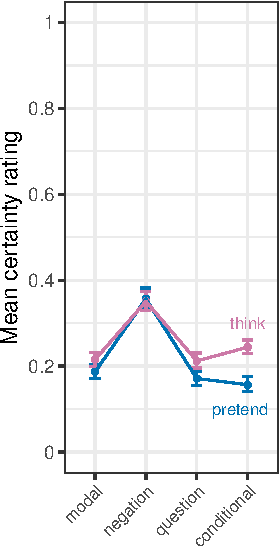
\includegraphics[width=.225 \textwidth, valign=T]{negation-high-1.pdf}
			&
			\vspace{-.6\baselineskip}
			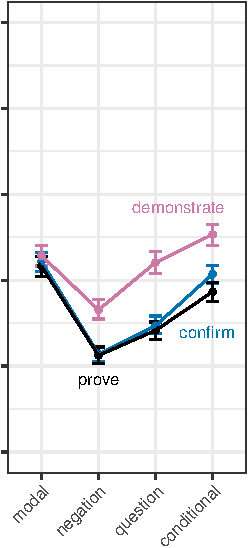
\includegraphics[width=.2\textwidth, valign=T]{negation-low-1.pdf}
			&
			\vspace{-.6\baselineskip}
			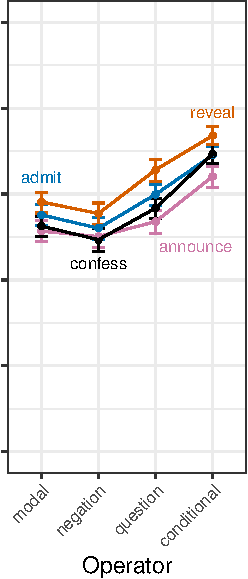
\includegraphics[width=.2\textwidth, valign=T]{conditional-high-1.pdf}
			&
			\vspace{-.6\baselineskip}
			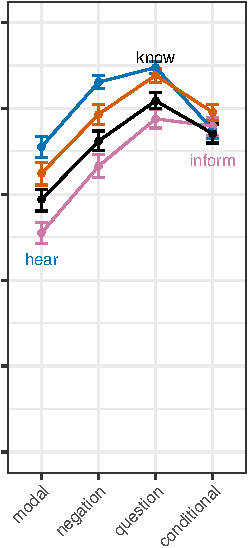
\includegraphics[width=.2\textwidth, valign=T]{modal-low-1.pdf}
			% &
			% \vspace{-.6\baselineskip}
			% 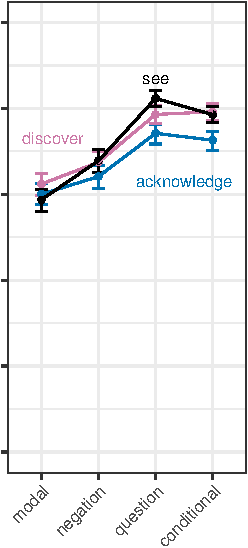
\includegraphics[width=.2\textwidth, valign=T]{discover-1.pdf}
			\\
		\end{tabular}
		% }
		
		\caption{Mean certainty ratings by operator with $95\%$ bootstrapped confidence intervals, for some groups of predicates (\lq predicate patterns\rq).}
		\label{fig:patterns}
	\end{figure}

	
	%
	The non-veridical predicates \emph{pretend} and \emph{think} exhibit the `Negation high' pattern, shown in panel (a) of Figure~\ref{fig:patterns}. These are the only predicates that are most projective under negation compared to all other operators. This could be related to 
	assumptions that non-veridical doxastics like \emph{think} can often be interpreted in comparison to a stronger veridical alternative (e.g., \citealt{heim_artikel_1991,chemla_epistemic_2008}). We tentatively hypothesize that this can lead to an inference that the CC is false in upward-monotone contexts, but not under negation. A similar alternative seems to be salient for \emph{pretend}, but not the non-veridical communicative predicates \emph{say} or \emph{suggest}.
	
	The inferential predicates \emph{confirm, demonstrate}, and \emph{prove} exhibit a `Negation low' pattern, shown in panel (b). These are most projective under modals and conditionals and least projective under negation. Here, we may hypothesize that a negative statement involving these predicates is often only taken as relevant (in a Gricean sense) when it is antecedently known that there was an attempt to confirm/demonstrate/prove the truth of the CC. This may result in an inference that this attempt failed and result in lower projection ratings under negation.
	
	For \emph{admit, announce, confess}, and \emph{reveal}, the CC is most projective when embedded in conditional antecedents: This `Conditional high' pattern (c) may suggest that the discourse effect of a conditional interacts with these change-of-state communication predicates.
	
	Finally, the predicates \emph{hear, inform,} and \emph{know} exhibit a `Modal low' pattern (d). The lexical meaning of these predicates, whose CCs are among the most projective, appears to interact with the modal adverb {\em perhaps}, yielding lower projection ratings.

\section{Conclusion}

\bibliographystyle{sub-chicago}
\bibliography{projection}



\newpage
\appendix

\section{20 clauses}\label{app:a-clauses}
    The contents of the following 20 clauses, which realized the complements of the 20 clause-embedding predicates, were investigated in Exps.~1-4:

    %\begin{multicols}{2}
    \begin{enumerate}%[leftmargin=3ex,itemsep=-2pt]
        \item Mary is pregnant.
        \item Josie went on vacation to France.
        \item Emma studied on Saturday morning.
        \item Olivia sleeps until noon.
        \item Sophia got a tattoo.
        \item Mia drank 2 cocktails last night.
        \item Isabella ate a steak on Sunday.
        \item  Emily bought a car yesterday.
        \item  Grace visited her sister.
        \item Zoe calculated the tip.

    %\columnbreak
        
        \item  Danny ate the last cupcake.
        \item  Frank got a cat.
        \item  Jackson ran 10 miles.
        \item  Jayden rented a car.
        \item  Tony had a drink last night.
        \item  Josh learned to ride a bike yesterday.
        \item  Owen shoveled snow last winter.
        \item  Julian dances salsa.
        \item  Jon walks to work.
        \item  Charley speaks Spanish.
            
    \end{enumerate}
    %\end{multicols}

\section{Consequents for conditional target stimuli in Exps.~4} \label{app:b-consequents}
    We created 20 consequent clauses for the three experiments in which the 20 clauses were embedded in the antecedent of a conditional (Exps.~4). Each of the 20 clauses was paired with a unique consequent clause, as shown in the list below. To minimize the variability of the effect of the contents of these consequent clauses on the projection of the contents of the 20 complement clauses, the consequent clauses all consist of a uniquely named subject and an adjectival predication in the future tense ({\em will be}), and the adjectives all denote an emotion. We selected the 20 emotion-denoting adjectives based on the valence and arousal values reported in \citealt{warriner_norms_2013}: 10 of the adjectives had a positive valence, and 10 had a negative valence; all 20 adjective had an arousal value between 4.7 and 6.5. 
    
    \begin{enumerate}%[leftmargin=3ex,itemsep=-2pt]
    
    \item \ldots that Mary is pregnant, Esther will be mad.
    \item \ldots that Josie went on vacation to France, Arnold will be frustrated.
    \item \ldots that Emma studied on Saturday morning, Liam will be proud.
    \item \ldots that Olivia sleeps until noon, Elijah will be embarrassed.
    \item \ldots that Sophia got a tattoo, Ariel will be giddy.
    \item \ldots that Mia drank 2 cocktails last night, Mariela will be worried.
    \item \ldots that Isabella ate a steak on Sunday, Liz will be delighted.
    \item  \ldots that Emily bought a car yesterday, Kate will be excited.
    \item \ldots that  Grace visited her sister, Henry will be surprised.
    \item \ldots that Zoe calculated the tip, Alex will be astonished.
    \item  \ldots that Danny ate the last cupcake, Harper will be disgusted.
    \item  \ldots that Frank got a cat, Lucas will be grouchy.
    \item  \ldots that Jackson ran 10 miles, Kayla will be cheerful.
    \item  \ldots that Jayden rented a car, Brittany will be furious.
    \item  \ldots that Tony had a drink last night, Victoria will be ashamed.
    \item  \ldots that Josh learned to ride a bike yesterday, Mason will be envious.
    \item  \ldots that Owen shoveled snow last winter, Bianca will be jealous.
    \item  \ldots that Julian dances salsa, Logan will be joyful.
    \item  \ldots that Jon walks to work, Caleb will be suspicious.
    \item  \ldots that Charley speaks Spanish, Jay will be happy.
    
    \end{enumerate}

\section{Control stimuli in Exps.~1-3}\label{app:c-control}

    The control stimuli in Exps.~1-3 were the contents of main clauses. In Exps.~1q, 2q and 3q, the control stimuli consisted of the polar questions in (1). The non-restrictive relative clauses (NRRCs), given in parentheses in (1), were included in Exps.~2q and 3q, where at-issueness was measured with an assent diagnostic. The control stimuli here consisted of two clauses (like the target stimuli), to allow the relevant speaker to assent with one of two clauses.

    \ex.[(1)] Sentences for control stimuli in in question embedding experiments (Exps.~1q, 2q and 3q)
      \a. Do these muffins (, which are really delicious,) have blueberries in them?
      \b. Does this pizza (, which I just made from scratch,) have mushrooms on it? 
      \b. Was Jack (, who is my long-time neighbor,) playing outside with the kids? 
      \b. Does Ann (, who is a local performer,) dance ballet?
      \b. Were John's kids (, who are very well-behaved,) in the garage?
      \b. Does Samantha (, who is really into fashion,) have a new hat?
      \z.
    \z.

    We expected participants to give low responses on the `certain that' diagnostic for the control stimuli in (1), indicating that the speaker is not certain of the main clause content, because main clause content is hypothesized to not project out of polar questions. These expectations were borne out, as shown in the third column of Table~\ref{t-controls} for Exps.~1q, 2q, and 3q. We also expected participants to give low responses on the at-issueness diagnostics for the control stimuli in (1), indicating that the main clause content is at-issue. These expectations were borne out for Exps.~1q and 2q, as shown in the fourth column of Table~\ref{t-controls}, but the ratings were higher than expected for Exp.~3q. See below for discussion.

    In the remaining experiments, the control stimuli consisted of the positive declarative variants of (1) given in (2). The NRRCs in parentheses were realized in Exps.~2 and 3 for the reason explained above, as well as in Exp.~1c, to make the control stimuli more similar to the target stimuli (which also consisted of two clauses, namely the antecedent and the consequent).

    \ex.[(2)]  Sentences for control stimuli in negation, modal and conditional embeddings
      \a. These muffins (, which are really delicious,) have blueberries in them.
      \b. This pizza (, which I just made from scratch,) has mushrooms on it. 
      \b. Jack (, who is my long-time neighbor,) was playing outside with the kids. 
      \b. Ann (, who is a local performer,) dances ballet.
      \b. John's kids (, who are very well-behaved,) were in the garage.
      \b. Samantha (, who is really into fashion,) has a new hat.
      \z.
    \z.

    We expected participants to give high responses on the `certain that' diagnostic for the control stimuli in (2), indicating that the speaker is certain of the main clause content, because speakers are hypothesized to be committed to the asserted main clause content. These expectations were borne out, as shown in the third column of Table~\ref{t-controls} for the `n', `m' and `c' variants of Exps.~1, 2, and 3. We expected participants to give low responses on the at-issueness diagnostics for the control stimuli in (2), indicating that the main clause content is at-issue. These expectations were borne out for the `n', `m', and `c' variants of Exps.~1, as shown in the fourth column of Table~\ref{t-controls}, but not for the `n', `m', and `c' variants of Exps.~2 and 3. See below for discussion.

    \begin{table}[h!]
        \centering
        \begin{tabular}{r r r r l }
            & &  \multicolumn{2}{c}{Mean ratings} &  \\ 
            Exp. & Control stimuli & Certainty & Not-at-issueness & At-issueness measure \\ 
            \hline
            1q & (1) & .14 & .05  & asking whether $c$ \\
            1n & (2) &  .95 & .04 & sure that $c$\\
            1m & (2) & .96 & .03 & sure that $c$\\
            1c & (2) with NRRC & .94  & .08 & sure that $c$\\
            \hline
            2q & (1) with NRRC & .18 & .07 & {\em yes}, $c$\\
            2n & (2) with NRRC& .96 & .22 & {\em yes, that's true}, $c$\\
            2m & (2) with NRRC& .96 & .25 & {\em yes, that's true}, $c$\\
            2c & (2) with NRRC& .96 & .22 & {\em yes, that's true}, $c$\\
            \hline
            3q & (1) with NRRC & .17 &  .28 & {\em yes}, but $\neg c'$\\
            3n & (2) with NRRC & .94 & .44 & {\em yes, that's true}, but $\neg c'$\\
            3m & (2) with NRRC & .93 & .50 & {\em yes, that's true}, but $\neg c'$\\
            3c & (2) with NRRC & .93 & .53 & {\em yes, that's true}, but $\neg c'$\\
            \hline
        \end{tabular}
        \caption{Mean certainty and at-issueness ratings for control stimuli, for self-declared American English participants}\label{t-controls}
    \end{table}

    As mentioned above, the mean at-issueness ratings were higher than expected in the `n', `m', and `c' variants of Exps.~2 and all four of the Exps.~3. We discuss these exceptions in more detail here because they allow us to further understand the various measures for at-issueness investigated in this paper. The example in (3a) illustrates the version of the assent diagnostic applied in Exps.~2n, 2m, and 2c: the assent particle {\em yes} is followed by the clause whose content is diagnosed, here, the content of the main clause. The related affirmation diagnostic applied in Exp.~2q (where the mean at-issueness rating was as low as expected) is illustrated in (3b).

    \ex.[(3)]
        \a. Sample control stimulus in Exps.~2n, 2m, and 2c
            \a.[A:] These muffins, which are really delicious, have blueberries in them.
            \b.[B:] Yes, that's true, they have blueberries in them.
            \z.
        Question to participants: Does A's response to B sound good?
        \b. Sample control stimulus in Exp.~2q
            \a.[A:] Do these muffins, which are really delicious, have blueberries in them?
            \b.[B:] Yes, they have blueberries in them.
            \z.
        Question to participants: Does A's response to B sound good?
        \z.
    \z.

    As shown in Table \ref{t-controls},  the group mean on the control stimuli is numerically higher (at .22 or .25) than for Exp.~2q (.07). We hypothesize that a possible explanation for this difference is that participants take A to assert both the content of the main clause and of the NRRC in (3a) but is only asking about the main clause content in (3b). Whereas B's affirmation in (3b) specifies the one content that is affirmed, B's assent in (3a) specifies only one of the two contents that A asserted, seemingly leaving out a specification of the second content, that of the NRRC. Participants may judge B's response in (3b) to be less acceptable than in (3a) because of this missing content specification. This hypothesis is consistent with the results of \posscite{syrett_experimental_2015} Exp.~3, which suggests that content of a sentence-medial NRRCs can be the target of a direct denial, though the main clause content is preferred as the target of such a denial. That the group means on the control stimuli in our Exps.~2n, 2m, and 2c are still relatively low may be due to the fact that the one content that was specified is the at-issue main clause content. One would expect lower acceptability ratings in a version of this diagnostic in which the one content that was specified is the NRRC.

    The mean at-issueness ratings for the control stimuli were also higher than expected in Exps.~3. The examples in (4) illustrate the versions of the affirmation and assent diagnostics used in these experiments:

    \ex.[(4)]
        \a. Sample control stimulus in Exp.~3q
            \a.[A:] Do these muffins, which are really delicious, have blueberries in them?
            \b.[B:] Yes, but they aren't really delicious.
            \z.
        Question to participants: Does A's response to B sound good?
        \b. Sample control stimulus in Exps.~3n, 3m, and 3c
            \a.[A:] These muffins, which are really delicious, have blueberries in them.
            \b.[B:] Yes, that's true, they but they aren't really delicious.
            \z.
        Question to participants: Does A's response to B sound good?
        \z.
    \z.

    The mean at-issueness rating for the control stimuli in Exp.~3q was comparatively higher (at .28) than for Exp.~1q (.05) or Exp.~2q (.07). We hypothesize that that this difference (especially to Exp.~2q) is due the content of the NRRC being directly denied, even though it was presented as backgrounded content in A's question (as shown in (2), the content of none of the other NRRCs was a matter of personal taste).

    The mean at-issueness ratings for the control stimuli in Exps.~3n, 3m, and 3c were numerically even higher than for Exp.~3q and, in fact, the highest across all 12 experiments (at .44, .50, and .53, respectively). There are two factors that could be implicated in the difference between Exp.~3q and Exps.~3n, 3m, and 3c: first, the NRRC is included in a polar question in the former but a declarative assertion in the latter; second, B utters an affirmation {\em yes} in the former but an assent {\em yes, that's true} in the latter. For instance, participants might judge B's direct denial of the content of the NRRC as less acceptable when A uttered a declarative assertion and B assented with that assertion using {\em yes, that's true} than when A uttered a polar question and B responded in the affirmative with {\em yes}. Both factors must be considered in future research on at-issueness measures.

\section{Participant information and data exclusion criteria}\label{app:d-participants}

    This supplement provides information on the participants of the 12 experiments and the criteria by which participants' data were excluded. The first three columns of Table \ref{t:exclusion} show, for each of the 12 experiments how many participants were recruited, their age range and mean age, and their self-reported gender; no gender data was collected in Exp.~1q. The next three columns provide information on the number of participants whose data were excluded based on the following criteria:
    
    \begin{itemize}%[itemsep=-2pt]
        
        \item `multiple': Due to an experimental glitch, some participants participated more than once in Exp.~1q. Since no information was available on which one was their first take, those participants' data was removed. 
        
        \item `language': Participants' data were excluded if they did not self-identify as native speakers of American English.
        
        \item `controls': Participants' data were excluded if their mean rating on the 6 main clause control items in the projection block was more than 2 sd above the group mean (in Exps.~1q, 2q, and 3q) or more than 2 sd below the group mean (in the remaining experiments). Participants' data were also excluded if their mean rating on the 6 main clause control items in the at-issueness block was more than 2 sd above the group mean (across all experiments).
         
        \item `variance': Participants' data were excluded if they always selected roughly the same point on the response scale for the target stimuli. To identify such participants, we first identified participants whose mean variance on the target stimuli was more than 2 sd below the group mean variance and then manually inspecting their response patterns. The data of participants who used the full scale was not excluded. 
        
    \end{itemize}

    The remaining columns of Table \ref{t:exclusion} provide information on the remaining participants, that is, the participants' data that entered into the analysis. Participants took around 9-11 minutes to complete the various experiments. Participants were paid more in Exps.~1c, 2c, and 3c than the remaining experiments because the target stimuli in those experiments were longer (as they consisted of conditionals). More women than men were recruited in many of the experiments because the experiments were run at a time when Prolific went viral on TikTok, resulting in a large number of young women registering for the service (around July 24, 2021; see \url{https://blog.prolific.co/we-recently-went-viral-on-tiktok-heres-what-we-learned/}, \\ last accessed February 4, 2022).  

    \begin{sidewaystable}[h!]
      \centering
      \begin{tabular}{l | r r r | r r r r | r r r | r }
      &  \multicolumn{3}{c|}{Recruited participants} & \multicolumn{4}{c|}{Exclusion criteria} & \multicolumn{3}{c|}{Remaining participants} &  \\ 
      Exp. & total & ages (mean) & gender (f/m/o/u) & multiple & language & controls & variance & total & ages (mean) & gender (f/m/o/u) & payment   \\ 
      \hline
      1q & 300  & 19-74 (38.2)  & --  & 5  & 7  & 35  & 0  & 242   & 21-74 (39.2) &  -- & \$1.70\\
      1n & 300  & 18-74 (33.2)  &  150/145/5/0 & 0  & 8 & 17 & 1 & 274  & 18-74 (33.3) & 141/128/5/0 & \$1.70\\
      1m & 300  & 18-74 (32.7) & 150/141/7/2  &  0 & 0  & 19 & 0   & 281   & 18-74 (32.7) & 144/129/7/1 & \$1.70 \\
      1c &  300 & 18-58 (25.9)  & 249/45/6/0 & 0 & 6  & 26 & 2  & 266  &  18-58 (24.8) & 235/25/6/0  & \$2.15 \\
      2q & 250  &  18-58 (25.5) &  201/43/6/0  & 0 & 4  & 24  & 1 & 220  & 18-58 (24.8)  & 187/28/5/0  & \$1.70 \\
      2n & 250  &  18-69 (33.2)  &  127/114/6/1 & 1  & 4  & 29 & 0& 215  &  18-69 (33.1) & 113/95/6/1    & \$1.70\\
      2m & 251  & 18-74 (31.7)  & 132/113/6/0  & 0  & 4  & 27 &  0 & 220  & 18-70 (31.9) & 116/98/6/0 & \$1.70\\
      2c &  250 &  18-56 (24.5)  & 212/30/8/0  & 0  & 0  & 26 & 0  & 224  & 18-56 (24.4) & 195/24/5/0 & \$2.15\\
      3q & 250  &  18-66 (32.4) &  140/102/7/1 &  0 & 4  & 20  & 0  &  225 & 18-66 (32.6) & 125/93//7/0  & \$1.70 \\
      3n & 250  &  18-70 (24.6) & 114/31/5/0  & 0  & 5  &  13 & 4  & 228  & 18-70 (24.3) &  198/25/5/0 &\$1.70 \\
      3m & 250  & 18-63 (25.5)  & 205/40/5/0 &  0 & 3  & 14 &  0 & 233  &  18-63 (24.8) & 197/31/5/0 &\$1.70 \\
      3c & 250  & 18-59  (27.5) & 182/64/4/0  & 0  & 3  & 17 & 0 & 230  &  18-59 (26.7)  & 177/49/4/0  & \$2.15\\
      \end{tabular}
      \caption{Recruited participants, excluded data, and remaining participants in Exps.~1, 2 and 3. Gender distinctions were `f' = female, `m' = male, `o' = other, and `u' = undeclared.}\label{t:exclusion}
    \end{sidewaystable} 

\end{document}
